\documentclass[resume]{subfiles}



\begin{document}
\section{Buildroot}
\subsection{Répertoires}
\begin{figure}[H]
\centering
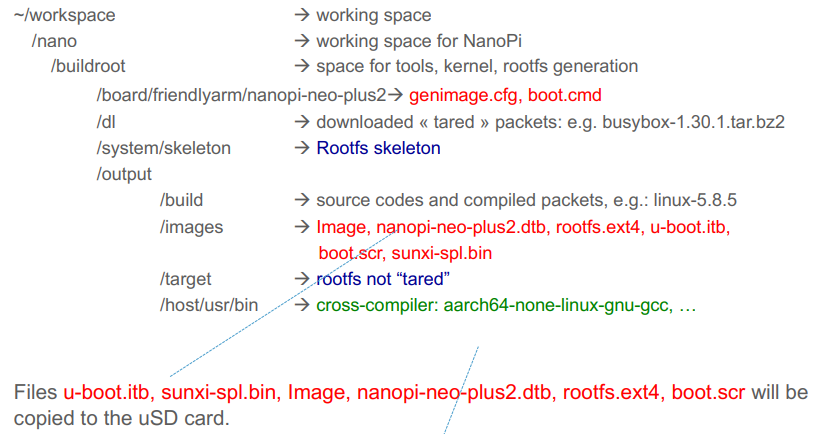
\includegraphics[width=\columnwidth]{img_1.png}
\end{figure}
Ce qui est manquant de le dossier output sera recompilé lorsque la commande \verb!make! est lancée (ou alors en faisant la commande \verb!make <package>-rebuild!.\\
Le dossier \verb!rootfs_overlay! permet d'ajouter des fichiers au \verb!rootfs!
(\verb!/workspace/nano/buildrootboard/friendlyarm/nanopi-neo-plus2/rootfs_overlay!)
\subsection{Compilation}
Dans le répertoire \verb!buildroot!, effectuer \verb!make menuconfig! puis \verb!make!. \verb!make clean! pour effacer tous les fichiers compilés.\\
La configuration permet notamment de 
\begin{enumerate}
\item Modifier le rootfs
\subsection{Carte SD}
\begin{figure}[H]
\centering
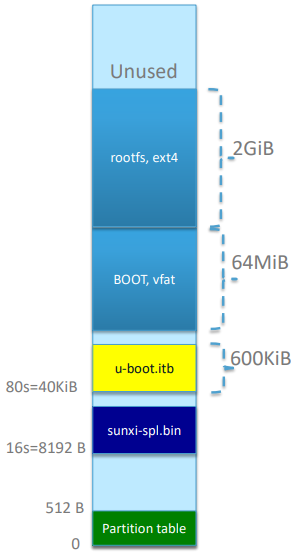
\includegraphics[width=3.00cm]{img_2.png}
\end{figure}
\begin{center}
\begin{tabular}{lccc}
Rootfs (ext4) & & 2GiB\\
BOOT, vfat / ext4 & & 64 MiB\\
U-Biit-itb & 80 & & 600KiB\\
sunxi-spl.bin & 16 & 79 & 32KiB\\
MBR (partition table) & 0 & 15 & 512B
\end{tabular}
\end{center}





\end{enumerate}



\end{document}